\chapter{Merkmalsextraktion}

\section{Verwendete Software}

Um die verschiedenen Verfahren zur Merkmalsextraktion zu vergleichen wurde ein Programm in C++ erstellt.
Also Entwicklungsumgebung wurde die freie und quellenoffene Software Eclipse verwendet.
Die genutzten Implementierungen der Bildverarbeitungsalgorithmen stammen aus der Bibliothek OpenCV. Hierbei handelt es sich um eine unter der BSD Lizenz veröffentlichten Software die sehr viele Methoden zur Bildverarbeitung und Maschinellem sehen enthält. \cite{cvlib}

\section{Hardware}

Das Programm wurde auf einem Laptop mit folgender Hardware erstellt und getestet:
\begin{itemize}
\item Intel Core i7-4720HQ mit bis zu 3.6 GHz
\item 8 GB DDR3L-SDRAM mit 1600 MHz
\item Nvidia Geforce GTX 960M
\end{itemize}

Als Kamera wurde eine Logitech HD Pro C920 Webcam verwendet, da diese sich durch ein sehr gutes Preis-Leistungs Verhältnis auszeichnet.

\section{Erstellte Software}
Zum testen und vergleichen der drei behandelten Merkmalsverfahren wurde ein Programm erstellt, das mit Hilfe dieser durch Bilder vorgegebene Objekte in dem Videostream einer Webcam erkennt.
Der verwendete Algorithmus lässt sich durch das setzen einer Variable bestimmen. Dies ist zwar nicht so benutzerfreundlich wie die Übergabe eines Arguments beim Aufruf des Programms, da bei jeder Änderung neu kompiliert werden muss, aber für Testzwecke ist es ausreichend.
Nachdem die Header-Dateien der benötigten Bibliotheken eingebunden wurden, werden die Bilder der zu suchenden Objekte aus einem definierbaren Ordner geladen. Es können theoretisch beliebig viele Bilder in diesen Ordner eingefügt werden, es wurden aber maximal 6 gleichzeitig getestet.
Da der Autofocus der Webcam nicht sehr zuverlässig funktioniert, wurde eine Manuelle Focus Funktion in Form einer OpenCV Trackbar Implementiert. 
\begin{figure}[h]
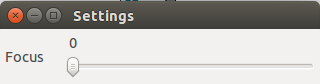
\includegraphics[width=0.6\textwidth]{trackbar.png}
\centering
\end{figure}
Um die Daten der Kamera verarbeiten zu können wird ein VideoCapture Objekt angelegt über das man die Mat-Container der einzelnen Frames beziehen kann.
Um die erkannten Objekte am besten Farblich darzustellen wird der Farbkreis in die Anzahl der zu erkennenden Objekte unterteilt. Das lässt sich am einfachsten im HSI Modell realisieren in dem jedes Objekt einen Hue wert:
\begin{equation}
H = i \cdot \dfrac{180}{\text{Anzahl der Objekte}} \\
\text{mit } 0 < i < \text{Anzahl der Objekte}
\end{equation}
Die so erhaltenen Farben werden anschließend in das RBG-Format umgerechnet und in einen Vektor für die spätere Verwendung gespeichert.
Da die Algorithmen auf Graustufenbildern arbeiten werden die Bilder der zu erkennenden Objekte konvertiert und in ein separates Array gespeichert.
Anschließend werden nach dem gewünschten Verfahren die Keypoints aus den Bildern extrahiert und die Deskriptoren berechnet.
Dies wird anhand der Methoden \emph{detect} und \emph{compute} der Klassen \emph{xfeatures2d::SIFT}, \emph{xfeatures2d::SURF} und \emph{ORB} bewerkstelligt. 
Falls bei diesem Schritt ein Fehler auftritt muss das betroffene Objekt in Form des zugehörigen Bildes, der Keypoints und der Deskriptoren aus den jeweiligen Vektoren gelöscht werden.
Dies ist insbesondere wichtig da die zu einem Objekt gehörenden Daten nur durch die Stelle in den Vektoren zusammenhängen.
Nachdem die Merkmale aus den Objektbildern extrahiert wurden, springt das Programm in eine nur durch die Beendung des Programms unterbrechbare Endlosschleife in der die aktuellen Frames der Webcam bearbeitet werden.
Das neueste Frame wird in Form eines Mat-Objekts erfasst und, wie die Bilder der darzustellenden Objekte, wird auch dieses in ein Graustufenbild verwandelt um anschließend die Merkmale in Form von Keypoints und Deskriptoren zu extrahieren.
Nachdem nun alle Merkmale aus den Objekt-Bildern und aus dem aktuellen Frame vorhanden sind, gilt es das Set aus Merkmalen jedes Objekts mit jenen des neuesten Frames zu vergleichen um mögliche Übereinstimmungen zu finden.
Hierzu wird als erstes von dem BruteForceMatcher (BFMatcher) aus OpenCV gebrauch gemacht. Dieser berechnet die Übereinstimmung der Merkmale anhand der Deskriptoren.
Da dieser aber noch viele falsche Matches ausgibt, werden diese anschließend noch anhand der von Lowe vorgestellten Methode gefiltert.
Es werden nur Matches bei denen das Verhältnis der Deskriptordistanzen (wie in 2.4 beschrieben, sagt diese Distanz aus wie unterschiedlich zwei Deskriptoren sind) des zweitbesten zum erstbesten Match kleiner als ein bestimmter Wert (in unserem Fall 0.9) sind beibehalten. 
Dies bedeutet in der Praxis dass es nur einen wahrscheinlichen Kandidaten für das Matching gibt und somit die Wahrscheinlichkeit einer Fehlzuweisung gering ist.
Die so erhaltenen Matches werden anschließend mit der OpenCV Funktion \emph{drawMatches} in das Bild eingezeichnet.
\begin{figure}[h]
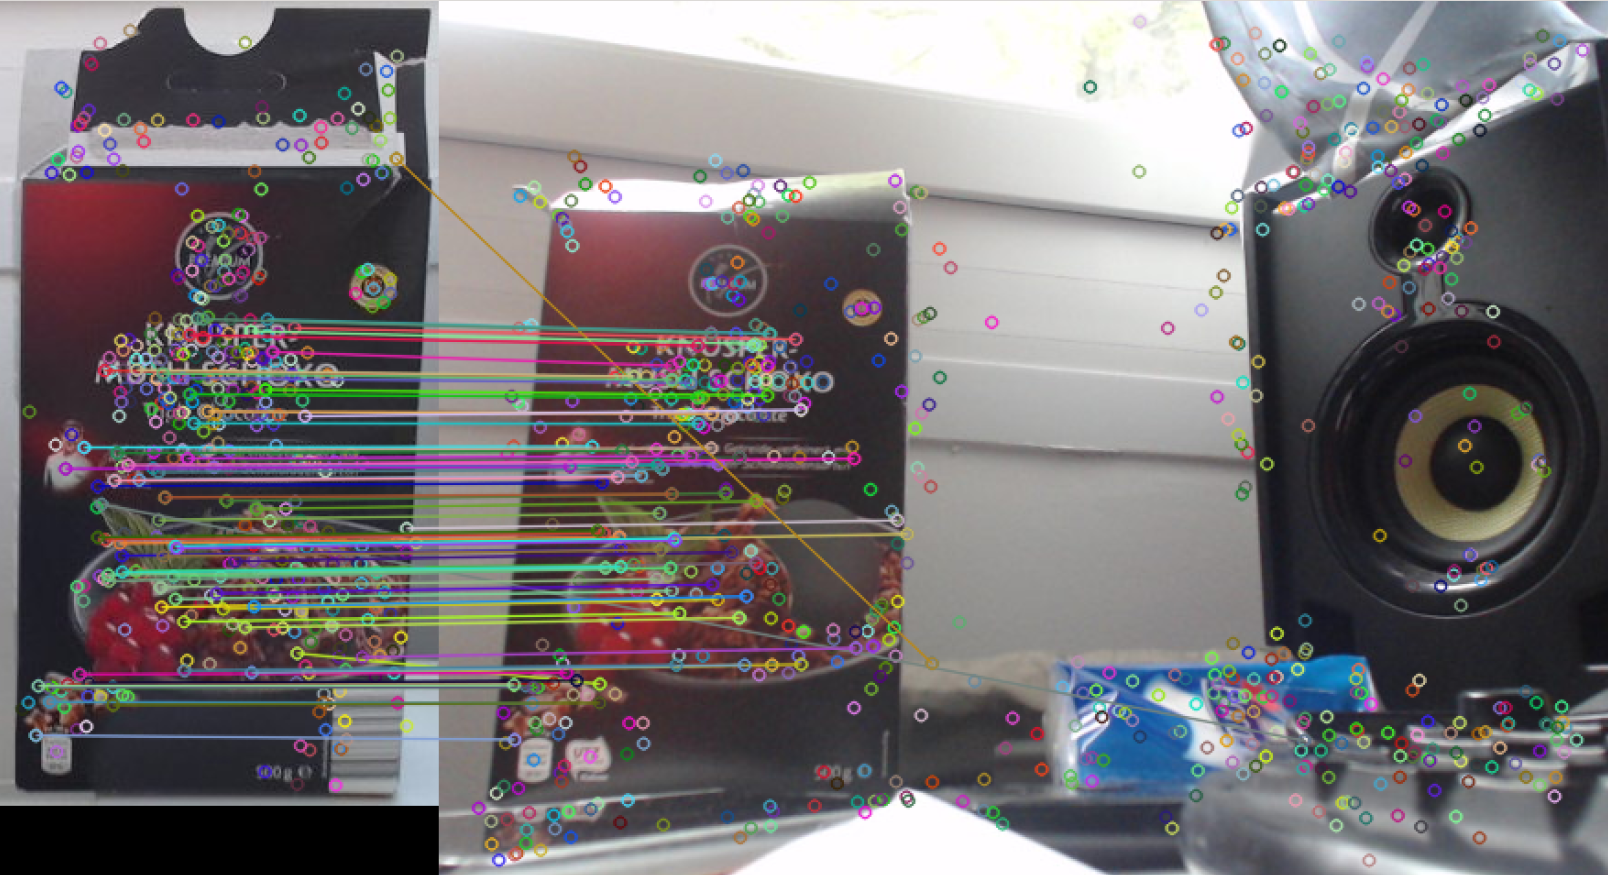
\includegraphics[width=0.8\textwidth]{matching.png}
\centering
\end{figure}
Anschließend wird aus den gefundenen Matches die Homographie, welche die Ausrichtung des gefundenen Objekts zu dessen hinterlegtem Bild beschreibt, berechnet.
Hierzu wird die OpenCV-Funktion \emph{findHomography} verwendet. Beim Aufruf dieser Funktion wird der Parameter \emph{method} übergeben, durch welchen man festlegen kann ob die Homographie herkömmlich berechnet wird oder mit Hilfe von RANSAC oder Least-Median die Ausreißer rausgefiltert werden.
Da die Punktemenge der wiedererkannten Keypoints aus der die Homographie ermittelt wird typischerweise Falschzuordnungen enthält, kommt die herkömmliche Methode nicht in Frage.
Bei Versuchen mit den beiden letzteren Methoden ergab sich RANSAC als die stabilere Variante und wird somit hier verwendet.
Mit der gefundenen Homographie-Matrix kann anschließend die Position des Objekts im aktuellen Frame ermittelt werden. Hierzu werden die Eck-punkte der hinterlegten Abbildung in einen Vektor gespeichert und samt der Homographie an die Funktion \emph{perspectiveTransform} übergeben. Diese liefert die Position der Eckpunkte im Frame, hierdurch ist die aktuelle Lage des Objekts bestimmt.
Mit Hilfe der Funktion \emph{line} wird eine Box um das gefundene Objekt gezeichnet.
\begin{figure}[h]
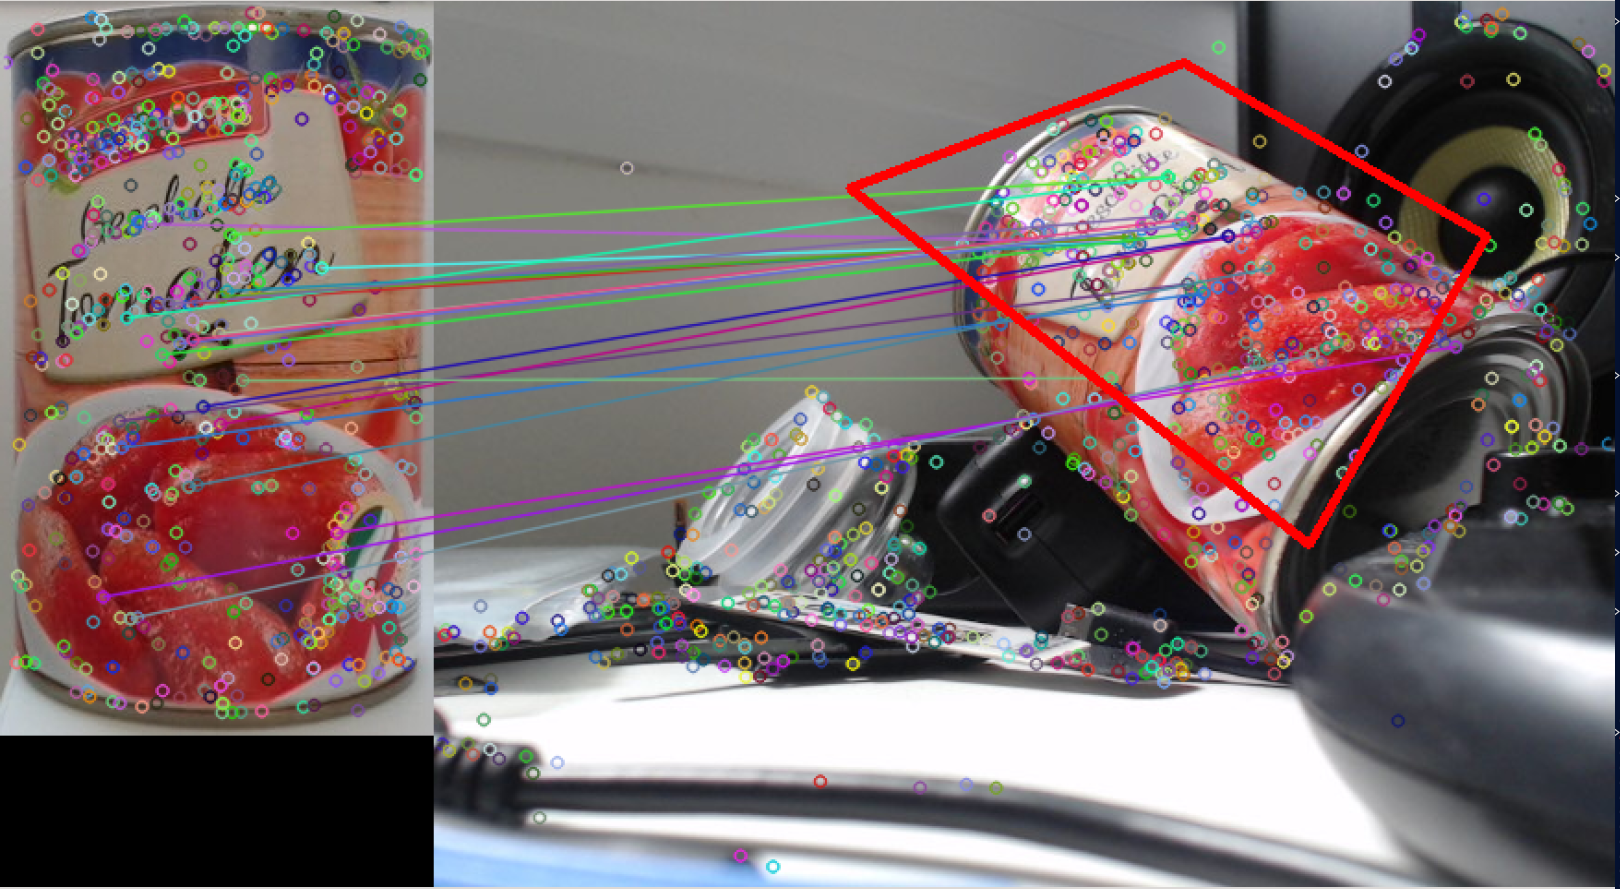
\includegraphics[width=0.8\textwidth]{homography.png}
\centering
\end{figure}

\subsection{GPU Beschleunigung}

Da die hier verwendeten Algorithmen zum Teil sehr rechenintensiv sind und auf dem Test-Laptop nicht alle Frames der Webcam verarbeitet werden konnten, wurde die Berechnung eines Teils der Operationen auf die GPU verlagert.
Dank der CUDA Bibliothek von NVIDIA und den Implementierungen der Bildverarbeitungsalgorithmen aus OpenCV die auf dieser basieren ist das relativ leicht zu realisieren.
Um die Bibliotheken nutzen zu können muss OpenCV samt den Plugins des \emph{contrib} Repository aus dem Quellcode kompiliert werden.
Zusätzlich zu den der üblichen \emph{Mat}, müssen hier \emph{cuda::GpuMat} Klassen verwendet werden.
Diese werden mit dem \emph{Mat} Bild initialisiert, somit wird dieses auf die Grafikkarte kopiert und es wird in der \emph{GpuMat} ein Pointer auf dieses gespeichert.
Anschließend können die Klassen \emph{cuda\:\:SURF\_CUDA} und \emph{cuda\:\:ORB} verwendet werden um die Berechnungen durchzuführen.
Für SIFT gibt es keine CUDA Implementierung, vermutlich aus patentrechtlichen Gründen.
Daher wurde versucht die SIFT Implementierung \emph{CudaSift} des Github Benutzers \emph{Celebrandil} in das Programm einzubauen.
Leider ist es nicht gelungen die Ausgangsschnittstellen dieser Bibliothek mit mit dem restlichen Programm zu verknüpfen.

\subsection{Benchmark}

Um die verschiedenen Methoden zu vergleichen wurden verschiedene Tests durchgeführt.
